\chapter{Requiring Change} % Chapter title
\label{chap:requiring} % For referencing the chapter elsewhere, use \autoref{ch:examples} 

In this chapter, I describe several systems that require interventions as a result of the increasing complexity of their environments.

\section{The Peril of Silos}
\label{sec:silos}

Academic disciplines are essential for the advancement of the sciences and the humanities.

Academic disciplines create rigor and discipline to help validate claims; to create a common language and framework; to share tools; and to build on the work of others in the same field to advance the field in effective ways. Academic journals, departments and conferences create vibrant communities that enable members of disciplines to collaborate and go deeper and deeper into a particular topic or domain.

Dividing academic and human endeavor into fields and disciplines, however, has a negative side-effect: it creates silos that make it difficult to work across, among, or beyond specific disciplines. Each discipline has its own frameworks and language, and even when they are saying similar things, it's often difficult to communicate effectively with people in other disciplines.

Siloing has multiple causes:

Peer review, which is important to ensure that claims are properly established and that the contributions that take up journals' limited space are in fact worthwhile, often reinforces depth over breadth. This ever increasing specialization often contributes to disciplines becoming more isolated and siloed. For example, In ``Looking Across and Looking Beyond the Knowledge Frontier: Intellectual Distance, Novelty, and Resource Allocation in Science,'' researchers describe a study that randomly assigned grant proposals to 2,130 evaluators. The study found that ``evaluators systematically give lower scores to research proposals that are closer to their own areas of expertise and to those that are highly novel'' \cite{boudreau2016looking}.

Also, scientific journals over time exhibit a tendency to evolve from publishing applied papers to papers that are more and more theoretical and abstract. In their paper ``The delineation of an interdisciplinary specialty in terms of a journal set'' researchers show that the interdisciplinary field of communications studies became increasingly self-referential as dedicated journals emerged \cite{leydesdorff2009delineation}.

\marginpar{Ed Boyden, a colleague at the Media Lab who runs the Synthetic Neurobiology group, often refers to the famous adage that the American philosopher, Abraham Kaplan, talks about as ``the principle of the drunkard's search'': \cite{kaplan2017conduct} drunks sometimes look for their lost keys under lampposts because that is where the light shines.}In addition, many departments often hire new academics and graduate students to advance existing departmental fields and disciplines, thus avoiding the risk of hiring people who might complicate peer review, tenure, or funding. In short, they are less adventurous.

Government funding tends to also be distributed along disciplinary lines, reinforcing the work done in existing disciplines and the silos around them.

The siloing that these various factors lead to can make disciplines more comfortable, but less creative. Ed Boyden, a colleague at the Media Lab who runs the Synthetic Neurobiology group, often refers to the famous adage that the American philosopher, Abraham Kaplan, talks about as ``the principle of the drunkard's search'': \cite{kaplan2017conduct} drunks sometimes look for their lost keys under lampposts because that is where the light shines. Boyden talks about the need to create flashlights --- metaphors for the tools he and his team are designing and building --- to facilitate a search for keys that have fallen in the dark areas between street lamps. It turns out that there are a lot of keys lying around in those dark spaces.

In fact, abundant evidence shows that the majority of useful inventions are discovered while looking for something else. A 2005 survey of European patents \cite{gambardella_value_2008} found that nearly half of the underlying inventions ``[arose] unexpectedly from research projects undertaken for other purposes or from activities other than inventing'' \cite{kennedy_opinion_2016}. \emph{The New York Times} reported on other studies with similar results.

Bridging disciplines is not a new idea. Interdisciplinary study has been widely and successfully pursued, generating new fields such as bioengineering, and unlocking tremendous value. New disciplines are often born at the intersection of old disciplines.

But as more and more cross-cutting fields such as computation emerge, we find that the the evolution of traditional disciplines may not be fast or flexible enough to deploy people and resources in the necessary fields to avoid being outpaced by technology, opportunities, and threats.

It is not only academia that is segmented and siloed. Corporations hit by the advances in the Internet have found themselves in completely new industries. For example, newspapers are competing with social networks, Craig's List, and mobile apps more than with other newspapers. Companies' IT strategies can no longer confine themselves to back rooms. Newspaper companies are having to learn about online video. Pharmaceutical companies are having to embrace artificial intelligence in the search for new drugs. At the same time, computer software companies are having to develop ethics policies.

\section{Monolithic and Centralized Systems}
\label{monoliths}

When Alexander Graham Bell invented the telephone, his business model was to lease out phones and hire contractors to run wires between them. The early telephone and telegraph companies strung wires from poles across the nation, controlling the entire network infrastructure, from local telegraph offices to the telephones. in people's parlors. This made sense when the technology was relatively simple, and controlling and managing the network centrally allowed it to evolve as the technology advanced.

When communications became digital, we entered a new age of communications infrastructure.

The digital age brought many advances in technology including better sound, and it also gave birth to encrypted phone calls and fax machines. Engineers working at Bell Laboratories soon realized that when they tried to make the quality of the sound better, they disrupted fax and other data services. David Isenberg, who was a Distinguished Member of Technical Staff at Bell Labs at the time, wrote the seminal paper, ``The Rise of the Stupid Network'' \cite{isenberg1997rise}, asserting that a network provider should not try to optimize its network for any particular purpose, but rather should diligently deliver the bits reliably from one end of the network to the other (creating an ``end-to-end'' network as it is sometimes called), and allow innovation to take place at the edges --- phone, fax and other services. They didn't take his advice, and not long after fired him.

\marginpar{Through government regulation, civil society, and technical advances and protocols designed by the technical community, the products and services were unbundled and broken up together with the layers of the Internet, allowing innovation and competition on each layer, greatly enhancing services to users, and lowering costs. A similar unbundling is now beginning in the financial services sector.}\dw{YY I think this is the only chapter with callouts. Remove them for consistency?}However, the regulators and the market began to ``unbundle'' the telecommunications system --- separating into layers what had once been offered as a bundle. This was the key to the success of the Internet. In Japan, for example, the Ministry of Posts and Telecommunications intervened to allow small Internet service providers to be licensed to provide Internet connectivity and forced deregulation to allow us to lease layer two connectivity from the telephone companies and sell IP services directly to consumers. Later, the Ministry went even further forcing telecommunications operators to lease dark fiber allowing me, for instance, to lease dark fiber and ``light up'' both ends with my own hardware and connect to the \ac{JPIX} directly by peering through the \ac{WIDE} network.

Other countries are still ``bundled.'' In the United Arab Emirates, for example, \ac{VoIP} is still banned by the nation's Telecommunications Regulatory Authority and all voice traffic is controlled by the local telecommunications companies. While the Internet architecture consists of technically unbundled layers, businesses continue to try to bundle the layers to exercise pricing and product power, but their arguments have much less technical validity than before the Internet.  Debates such as the current one over net neutrality in the United States are over the commercial bundling of layers.

Encryption created new issues, complicating, for instance, the ability of U.S. law enforcement authorities to order wiretaps. Many believed that encrypting communications would decrease surveillance because wiretaps would be harder, and for that reason the government fought to ban encryption., while many of us fought for end-to-end encryption. Once it became clear that the government would not win the debate, in 1994 it passed the \ac{CALEA} that funded the development of, and mandated the deployment of, digital wiretapping technologies at the telephone companies. This paved the way for wiretapping at the massive scale revealed by Edward Snowden two decades later. This was a very frustrating event for us, and a lesson that even in a decentralized, layered system, regulators can take their interventions to another layer to get what they want.

Through government regulation, civil society, and technical advances and protocols designed by the technical community, the products and services were unbundled and broken up, together with the layers of the Internet, allowing innovation and competition on each layer, greatly enhancing services to users, and lowering costs. (This argument is more fully described in \autoref{decentralization}.)

A similar unbundling is now beginning in the financial services sector. The United Kingdom through the second Payments Services Directive (PSD2) is compelling banks to open their data in a standardized format to allow others to create products and services on top of existing financial institutions \cite{cortet2016psd2}. The new directive, called Open Banking, came into force on January 13, 2018 \cite{manthorpe_what_nodate}. The Monetary Authority of Singapore is pushing for a similar Open Banking initiative \cite{banking_singapore_2017}.

Unbundling fundamentally changes the ability of new entrants to come into the marketplace of both ideas and businesses, increasing the number of competitors and the amount of competition. As the telecommunications layer based on this unbundled system became more successful, it began to affect the next layer on the ``stack'' --- the layer of media and and the public sphere that was originally built on top of the older monolithic communications technologies. (See \autoref{layertable} in \autoref{decentralization}.)

\section{Emergent Democracy}
\label{emergentdemo}

As unbundling and the Internet drove down the cost of communication, it allowed everyone to become a publisher and a contributor to the global dialog. This dramatically impacted the nature of media and the public sphere.

\marginpar{We believed that blogs would evolve into a social medium that would transform democracy and make the world a wonderful, new place.}In 2003, I wrote an essay with the active participation of my online community as weblogs, or blogs, began to flourish \cite{1Emergen42:online}. Ross Mayfield who participated in these conversations coined the phrase ``emergent democracy'' to described what we believed was a new form of democracy emerging from our new tools. We believed that blogs would evolve into a social medium that would transform democracy and make the world a wonderful, new place. 

What follows is the first part of the essay, in which I described emergent democracy. As you will see, It was prescient about some things and quite naive about others. It serves as a marker in time, reminding us of how transformative we hoped and believed the Internet's decentralized architecture would be. (I have excluded the remainder of the essay because it deals primarily with the specifics of the tools that we had available back in 2003.)

\textit{Essay except begins here.}

\begin{quote}
Proponents of the Internet have committed to and sought for a more intelligent Internet where new democratic methods could be enabled to help rectify the imbalance and inequalities of the world. Instead, the Internet today is a noisy environment with a great deal of power consolidation instead of the level democratic Internet many envisioned.

In 1993 Howard Rheingold wrote \cite{rheingold1993virtual},
\begin{quotation}
We temporarily have access to a tool that could bring conviviality and understanding into our lives and might help revitalize the public sphere. The same tool, improperly controlled and wielded, could become an instrument of tyranny. The vision of a citizen-designed, citizen-controlled worldwide communications network is a version of technological utopianism that could be called the vision of ``the electronic agora.'' In the original democracy, Athens, the agora was the marketplace, and more --- it was where citizens met to talk, gossip, argue, size each other up, find the weak spots in political ideas by debating about them. But another kind of vision could apply to the use of the Net in the wrong ways, a shadow vision of a less utopian kind of place --- the Panopticon.
\end{quotation}
\marginpar{``It is also possible that new technologies will empower terrorists or totalitarian regimes. These tools will have the ability to either enhance or deteriorate democracy and we must do what is possible to influence the development...''}

Since then he has been criticized as being naive about his views \cite{rheingold2001virtual}. This is because the tools and protocols of the Internet have not yet evolved enough to allow the emergence of Internet democracy to create a higher-level order. As these tools evolve we are on the verge of an awakening of the Internet. This awakening will facilitate a political model enabled by technology to support those basic attributes of democracy which have eroded as power has become concentrated within corporations and governments. It is possible that new technologies may enable a higher-level order, which in turn will enable a form of emergent democracy able to manage complex issues and support, change or replace our current representative democracy. It is also possible that new technologies will empower terrorists or totalitarian regimes. These tools will have the ability to either enhance or deteriorate democracy and we must do what is possible to influence the development of the tools for better democracy. This sentence also from 2003 sounds both prescient and naive.

\subsubsection{Democracy}

In the dictionary definition, democracy ``is government by the people in which the supreme power is vested in the people and exercised directly by them or by their elected agents under a free electoral system.'' In the words of Abraham Lincoln, democracy is a government ``of the people, by the people, and for the people'' \cite{lessig2002future}.

Rome and most democratic nations since then have chosen a republican form of representative democracy. Direct democracy does not scale and because the uneducated masses were considered unfit to rule directly, those who were more ``fit to lead'' were chosen to represent the masses. Representative democracy also allows leaders to specialize and focus in order to formulate opinions about the variety of complex issues, which need to be resolved where an uneducated and uninterested population could not be expected to directly understand all of the issues.

The failure of democracy to scale is also not complicated to understand. The founding fathers of this country, the ``egalitie, fraternitie and libertie'' of France and most other liberals that moved society toward freedom and liberty in the 1700's could not have been expected to visualize the growth of populations, radical evolution of science, vast increases of technology and incredible increases in mobility of information, money, goods, services and people. Nor could they know or visualize the topography of countries such as the United States, Canada and China, or continents such as Africa, Northern Europe, Russia or Latin America. They laid out such vast topography to the best of their ability on grids that bore no resemblance to the reality of the environment or to the huge increases in scale of population commerce and government. In the main, they did not foresee a need for the right to self-organize --- to adjust scale and degrees of separation as such increases occurred \cite{deehockjoiitoweb}.

As the issues facing government become larger and more complex, new tools are enabling citizens to self-organize more easily. It is possible that such tools will enable democracies to scale and become more adaptable.

A democracy is ideally governed by the majority and protects the rights of the minority. For a democracy to perform this properly it must support a competition of ideas, which requires critical debate, freedom of speech and the ability to criticize power without fear of retribution. In a true representative democracy the power must be distributed into multiple points of authority to enable checks and balances.

\subsubsection{Competition of ideas}

A competition of ideas is essential for a democracy to embrace the diversity of its citizens and protect the rights of the minority, while allowing the consensus of the majority to rule. The competition of ideas process has evolved with the advancement of technology.

For example, the printing press made it possible to provide more information to the masses and eventually provided the people a voice through journalism and the press. Arguably, this has been replaced by the voice of mass media operated by large corporations. As a result, there is less diversity and more internalization of the competition of ideas.

\subsubsection{Critical debate and freedom of speech}

The competition of ideas requires critical debate that is widely heard. Although we have many tools for managing such debate, increasingly there are barriers to our engaging in it at all.

\marginpar{In the increasingly sophisticated world of databases and systematic profiling of individuals, the protection of those citizens and whistleblowers willing to question power must be assured.}

\subsubsection{The Commons}

\begin{quotation}If nature has made any one thing less susceptible than all others of exclusive property, it is the action of the thinking power called an idea, which an individual may exclusively possess as long as he keeps it to himself; but the moment it is divulged, it forces itself into the possession of every one, and the receiver cannot dispossess himself of it. Its peculiar character, too, is that no one possesses the less, because every other possesses the whole of it. He who receives an idea from me, receives instruction himself without lessening mine; as he who lights his taper at mine, receives light without darkening me.

That ideas should freely spread from one to another over the globe, for the moral and mutual instruction of man, and improvement of his condition, seems to have been peculiarly and benevolently designed by nature, when she made them, like fire, expansible over all space, without lessening their density in any point, and like the air in which we breathe, move, and have our physical being, incapable of confinement or exclusive appropriation \cite{jefferson1813letter}.
--- Thomas Jefferson
\end{quotation}

As the notion of intellectual property continues to grow in scope, more and more of what was one part of common knowledge is becoming the property of corporations.

As the infrastructure for communication becomes more tuned to the protection of property than the free spreading of ideas, the capacity for critical debate is severely constrained.

Even though ideas are not subject to copyright, increasingly draconian copyright protection legislation limits the scope and meaning of fair use and even the flow of innovation, thereby having the same effect as if ideas were property owned and controlled by corporations. It includes the code inside of the computers and networks, which controls the transmission or reproduction of information.

\subsubsection{Privacy}

Democratic or otherwise, rarely, very rarely, does any concentration of power or wealth desire to see subjects well informed, truly educated, their privacy ensured or their discourse uninhibited. Those are the very things that power and wealth fear most. Old forms of government have every reason to operate in secret, while denying just that privilege to subjects. The people are to be minutely scrutinized while power is to be free of examination \cite{deehockjoiitoweb}.

In addition to the legal and technical ability to speak and engage in critical debate, citizens must be allowed to speak without fear of retribution. In the increasingly sophisticated world of databases and systematic profiling of individuals, the protection of those citizens and whistleblowers willing to question power must be assured. The powerful are increasingly able to threaten the weak, and this power must be countered by an increase in the ability of people to manage their identities, which are more and more defined by the profiles created by electronically collected information.

It is essential to understand the difference between privacy and transparency. When the powerful collect information to control the weak and hide behind secrecy, this is an invasion of privacy and is the basis of a surveillance-based method of security.

In one of the earliest critiques of the ID card proposal (January 1986) Professor Geoffrey de Q Walker, now dean of law at Queensland University, observed \cite{davies_privacy_nodate}:

\begin{quotation}One of the fundamental contrasts between free democratic societies and totalitarian systems is that the totalitarian government [or other totalitarian organization] relies on secrecy for the regime but high surveillance and disclosure for all other groups, whereas in the civic culture of liberal democracy, the position is approximately the reverse.\end{quotation}

Steve Mann presents the notion of sousveillance \cite{mann2002sousveillance} as a method for the public to monitor the establishment and provide a new level of transparency. This has been the role of the press, but with its strong orientation toward positive feedback, the media has tended to focus on less relevant issues, which get an inordinate amount of attention. One such example was the media's fascination with Gennifer Flowers and her claim that she had had an affair with President Clinton.

Weblogs and other forms of filtering coupled with many of the capture and transmission technologies discussed by Mann may provide a better method of capturing and filtering relevant information while suppressing irrelevant information where the privacy damage exceeds the value to the public.
An example of weblogs exceeding the ability of the mass media to identify relevant information is the case of Trent Lott. The national media covered briefly his racist comments during Strom Thurmond's 100th birthday party. After the national media had lost interest, the weblogs continued to find evidence of Lott's hateful past until the mass media once again took notice and covered the issue in more depth \cite{shachtman2002blogs}.

The balance between what is relevant and not relevant is exceedingly difficult and important and culturally biased. Mechanisms to check the filtering mechanism for corruption and imbalance are necessary. It will be a variety of checks and balances and the combination of a diversity of methods that may provide us with the balanced view.

\subsubsection{Polling and Direct Democracy}

Direct democracy - the government of the public by itself - has always been said to be impossible on a large scale because of the technical difficulty of such direct governance and the fact that the complexities of involved in running a large state requires a much deeper understanding of the issues, specialization, and a division of labor. Representative democracy, wherein elected representatives of the people are chosen through a voting mechanism, is considered by most to be the only possible way to manage a large democracy.
As the voting mechanism becomes more organized and the difficulty of participating in the critical debate increases, we find that elected representatives represent people who have the power to influence the voting mechanism and the public debate. These groups of people are often minorities who have more financial influence or the ability to mobilize a large number of motivated people through religious or ideological means. The extremists and corporate interests dominate many democracies, and the silent majority have very little input in the selection of representatives or the critical debate \cite{rebuildjoiito}.

A variety of groups have been successful in polling the silent majority and amplifying its opinions to provide support for moderate politicians on policy issues. One such group, Peaceworks, operates in Israel and Palestine through polling, by telephone and the Internet, the average citizens who are in favor of peace and amplifying their opinions by then publishing the results in reports and the mass media. This method of bypassing the traditional methods of influencing representatives is a form of direct democracy, which is becoming increasingly popular and important as technology makes such polling easier.

Generally, polling, as a form of direct democracy is very effective for issues which are relatively simple and about which the silent majority have an opinion that is under-represented. For more complex issues, such direct democracy is criticized as populist and irresponsible.

To address this issue, Professor James S. Fiskin has developed a method of polling called deliberative polling. Deliberative polling combines deliberation in small group discussions with scientific random sampling to increase the quality and depth of the understanding of the participants while maintaining a sampling that reflects the actual distribution of the population rather than the distribution of political power. Deliberative polling has been used successfully to poll people about relatively complex issues such as tax policies \cite{fishkin2000deliberative}.

It is possible that there is a method for citizens to self-organize to deliberate on and address complex issues as necessary and enhance our democracy without any one citizen being required to know and understand the whole. This is the essence of an emergence, and it is the way that ant colonies are able to ``think'' and our DNA is able to build the complex bodies that we have. If information technology could provide a mechanism for citizens in a democracy to participate in a way that allowed self-organization and emergent understanding, it is possible that a form of emergent democracy could address many of the complexity and scalability issues facing representative governments today.

In complex systems the role of the leader is not about determining the direction and controlling the followers, but about maintaining integrity, representing the will of the followers and influencing and communicating with peers and leaders above \cite{FuturePo61:online}. The leader becomes more of facilitator and a custodian of the process than a power figure, and is often the catalyst or manager of a critical debate or the representative of a group engaged in one \cite{Leadersh1:online}. The leader is often the messenger delivering the consensus of a community to another layer or group. Indeed, some leaders in a representative democracy act in this manner. And as leadership becomes necessary to manage the development of an opinion or idea about a complex issue, information technology could enable quick and ad hoc leader selection and representation of that opinion or idea in a larger debate. 
\end{quote}

\textit{End of essay excerpt.}


\subsubsection{Postscript to Emergent Democracy}

\textit{Thoughts from 2018} \\


\marginpar{What we imagined, but weren't able to build, were systems of leadership, institution building and collaboration --- or what to do after established institutions are overthrown.}Through our participation in and understanding blogs and early user-generated-content, we had predicted the rise of a new form of voice and collective action and the role of social media on politics and opinion.

This essay was written in 2003 before the Arab Spring that began in 2010 with the Tunisian Revolution, spreading to Libya, Egypt, Yemen, Syria and Bahrain. The success of the Arab Spring in overthrowing regimes was attributed in great part to the use of social media. The Arab Spring demonstrated that these emergent systems could help overthrow established institutions.

What we imagined, but weren't able to build, were systems of leadership, institution building and collaboration --- or what to do after established institutions are overthrown. While the Arab Spring was able to overthrow the dictatorships in Tunisia, Libya and Egypt, the activists were not well equipped to take over the operation of the government, and only Tunisia has resulted in a transition to a constitutional democracy \cite{ruthven2016understand}.

More recently, polarization, hate groups, and extremism on the Internet have been become exceedingly influential in the political sphere, many focused on attacking established power, institutions and the elite.

I believe that unlike the civil rights movement, which had developed an institutional structure and carefully constructed organizations to follow through with strategy and law-making, many of the online movements are still impulsive. For example, Martin Luther King Jr. read  Mahatma Gandhi's works and corresponded with Gandhi's associates and discussed nonviolent protest strategy \cite{reddick}. However, examples such as the TimesUp Movement and the Parkland students protesting gun violence show a much greater degree of organization, strategy and focus, clearly learning from the past and developing new techniques, while remaining decentralized organizations that lack clear leaders or leadership structures.

As the public sphere and democracy are being disrupted and reinvented, we face similar challenges --- an imperative --- in health.

\section{Rethinking Health and Medicine}
\label{requiringhealth}

Recent advances in systems biology, neuroscience, immunology, gut microbiology, and many other related fields reveal that the human health system is far more complex than we previously understood. The nervous system, the immune system and microbial systems within the body are all highly interconnected and complex --- and different for each person. We do not fully understand how these systems work, and much of our understanding is reductionist and inaccurate. Treatment paradigms are based on models that identify target problems in an effort to identify and develop molecules that can be deployed into a patient to intervene in his or her biological system to solve a problem. The model for research has essentially been a method akin to trial and error, and approval for use of new treatments in human beings has required a series of trials demanding a tremendous amount of time and money, as stipulated by government. \marginpar{Despite new developments and huge investments, the pharmaceutical, health care and insurance industry is losing billions of dollars on complex, unpredictable and a largely unsuccessful drug development, clinical trial and research ecosystem that is unable to keep up with the new challenges and opportunities.}Pharmaceutical drug development mostly conducted in an ecosystem dominated by large monolithic incumbents regulated by government agencies has remained relatively unchanged for the last 30 years. Early discovery experiments, performed in vitro or in cell culture assays, are followed by translational studies in various animal models and then by clinical trials. The process is further slowed by the fact that performance in one model system doesn't necessarily generalize to the others, so that molecules that seem promising in in vitro models often drop out as they move through the development chain.

Despite new developments and huge investments, the pharmaceutical, health care and insurance industry is losing billions of dollars on its complex, unpredictable and largely unsuccessful drug development procedures that are unable to keep up with the new challenges and opportunities as our new research and technology is revealing just how vastly complex organic life is:

\begin{enumerate}
\item Systems biology, network medicine and bioinformatics approaches have been predominantly used for analyses and interpretation of medical data but have limited applicability at scale \cite{devita2015death}. For example, Vincent DeVita in \textit{The Death of Cancer} argues that the combinatorial complexity of cancer treatments make it impossible to understand at scale.
\item Biomarker discovery, automation of research tasks, diagnoses of medical images, clinical data and several other areas would likely benefit significantly with integration of emerging technologies such as machine learning and \ac{AI} (See \autoref{fig:drugai}), gene editing and the ``-omics,': the emerging fields that include genomics, transcriptomics, epigenomics, proteomics, and metabolomics.
\item Phase 3 outcomes trials conducted by large biotech companies are among the most complex experiments performed in medicine. Around fifty percent of Phase 3 trials fail. In the U.S. Food and Drug Administration's recently published white paper, ``22 case studies where Phase 2 and Phase 3 trials had divergent results'' \cite{22CaseSt45:online}, a common theme is the difficulty of predicting clinical results across a wide patient base, even with the backing of solid data. 
\item The mechanism of action for many candidate drugs and biologics remains unknown. This knowledge is key to the design and discovery of effective therapeutics.
\item Clinical trials are expensive and lack learnings and predictions that could be gathered from past experimental successes and failures of candidate molecules, adverse events and \ac{$IC_{50}$}\footnote{$IC_{50}$ is the half maximal inhibitory concentration and is used to measure the potency of a substance in inhibiting a specific biological or biochemical function.} measurements.
\end{enumerate}


We are discovering how complex and interconnected every system inside of our body is as well as how much our health is connected to every system outside of our bodies. Health is, at a different scale, very similar to the geological ecosystem which is also a massively complex system of interconnected systems.

\begin{figure}[h]
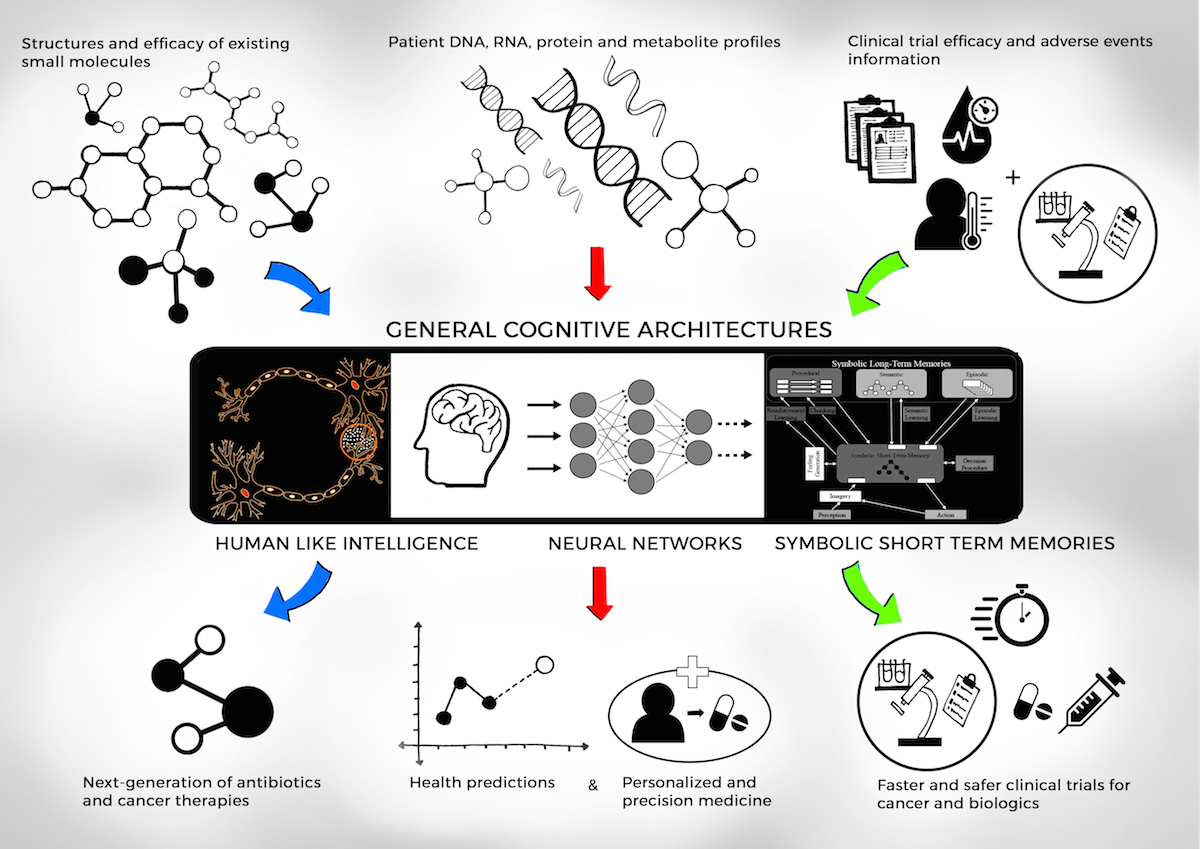
\includegraphics[width=\linewidth]{pictures/AI_DD-pratik}
\caption{Machine learning and artificial intelligence architectures for drug development. \cite{shahmlimage}}
\label{fig:drugai}
\end{figure}

\section{The Environment}
\label{sec:2environment}

In retrospect, it is clear that unbridled capitalism with a lack of feedback about what was happening to the environment has gotten us into the mess we call climate change. We had neither the measurements nor people properly positioned necessary for us to become aware of climate change and do something about it. \ac{NASA} even tried to stifle disclosure as the first climate scientists became aware of the issue \cite{winters2008investigative}. We now have a preponderance of evidence, but we are still at a loss as to how we're actually going to mitigate the worst effects of climate change, even as we watch them coming.

Most of our systems are designed to do things better and more efficiently without consideration for the costs and negative impacts that they are able to externalize, encouraged by the financial markets that reward the players who scale to create what consumers want to buy. These dynamics have led us to extract and consume so much of our natural resources with so little thought about the waste we are expelling back into the environment. 

We cannot expect the market to correct this on its own for it isn't set up to self-regulate or internalize these externalities. So I am currently working with my \ac{DCI} group and collaborators at the Emerson Collective on a way to account for ``natural capital',' adding to corporate balance sheets the value of the resources they use and the cost of the pollution they create. The aim is to make businesses put a price on their creation of what the British ecologist Garrett Hardin labeled ``The Tragedy of the Commons'' \cite{hardin1968tragedy}. We are exploring whether the blockchain or cryptography can help with the accounting of these types of assets and liabilities.

One concrete example is the use of carbon credits to create quotas on how much carbon companies put into the atmosphere, and allowing them to trade these credits to buy and sell savings in carbon emissions. The plan is to make a market for carbon emissions and other natural assets and liabilities that will help slow the exploitation of the natural systems. However, this is dealing mostly with ``stocks'' and some ``flows,'' to use words from systems dynamics.

Climate is, however, a highly complex system, and we are only measuring those elements that we know to monitor. James Hansen, an atmospheric physicists at the \ac{NASA} in the 1980s showed that key factors such as CO\textsubscript{2} and green house gases contribute to global warming \cite{hansen1981climate}, connecting fossil fuel emissions to climate change. My concern is that while greenhouse gases are clearly significant, it is easy to focus on only the most obvious and measurable elements of complex systems. We may be too focused on the atmosphere or on specific measurable parameters. 

Also, optimizing for any one variable can have unpredictable consequences in the long run. For example, biofuels which have been touted as an environmentally friendly alternative to fossil fuels, might have an opposite effort. Scientists argue that the production of ethanol from corn requires more fossil fuel energy \cite{patzek2004thermodynamics} the ethanol's energy value. In addition, the farming and processing methods are damaging the soil and causing other environmental side effects such as N\textsubscript{2}O release \cite{crutzen2007n}.

We need to adopt a systems approach to climate change. It is possible, if not likely, that the fundamental change that we need is a cultural intervention to redirect the sensibilities and behavior of consumers so that they spend money on products created with little negative impact on the environment...or, better, products created in ways that increase the sustainability of the planet.

Economists often say, ``\textit{when} the people in China and India are consuming as much energy and generating as much carbon per capita as Americans…'' rather than ``\textit{if} the people in China and India are consuming as much energy and generating as much carbon…'' Changing the norms of society may have more effect on the overall outcome than any accounting or policy change. Maybe we should promote a ``natural dream'' instead of the American Dream. 

It is also possible to change norms through policy interventions. Cars like the Toyota Prius and the Tesla are succeeding in part because of government subsidies to buyers and manufacturers. The success of these cars appear to be having an impact on norms.

Climate change is a complex global problem that is also local. Every town and village has a different context: ts energy requirements, its social dynamics, its industries and their impact on the local environment. Yet the architecture of markets and legal systems are often at state, national or even global scales. Change at a local level requires a bottom-up approach that can be coordinated but not literally managed in the traditional top-down fashion.

We need a social movement.

We need a theory of change --- a theory of the activation of communities. 